\chapter[Materiais e Métodos]{MATERIAIS E MÉTODOS}

Este capítulo descreve as Etapas 1 a 4 do processo KDD e o protocolo experimental utilizado na Etapa 5. Todo o trabalho foi desenvolvido em Python, com as bibliotecas \texttt{numpy} 2.5.4, \texttt{pandas} 3.0.6, \texttt{scikit-learn} 1.9.1 \citep{pedregosa2011scikit}, \texttt{scipy} 1.18.1, \texttt{matplotlib} 3.11.2 e \texttt{seaborn} 0.13.2. A mineração foi implementada em dois \textit{scripts} e reproduzida e expandida em um \textit{notebook}, que confere automaticamente os seus números contra os arquivos CSV gerados pelos \textit{scripts}:

\begin{itemize}
    \item \texttt{kdd\_breast\_cancer\_wisconsin.py}: experimentos com o Breast Cancer Wisconsin;
    \item \texttt{kdd\_wine.py}: experimentos com o Wine;
    \item \texttt{trabalho2\_kdd\_breast\_cancer\_wine.ipynb}: \textit{notebook} com as sete etapas do KDD e as análises complementares.
\end{itemize}

\noindent Todas as execuções utilizam sementes aleatórias fixas.

\section{ETAPA 1: COMPREENSÃO DO PROBLEMA E HIPÓTESES}

O problema consiste em medir quanto da estrutura das classes pode ser recuperado com diferentes níveis de supervisão. Para que a Etapa 6 pudesse confirmar ou refutar as expectativas iniciais de forma objetiva, cada hipótese foi formulada junto com um critério de verificação, conforme a Tabela \ref{tab:hipoteses}.

\begin{table}[htbp]
\centering
\caption{Hipóteses formuladas na Etapa 1 e critérios de verificação.}
\label{tab:hipoteses}
\footnotesize
\begin{tabular}{p{0.6cm} p{6.4cm} p{7.2cm}}
\toprule
\textbf{\#} & \textbf{Hipótese} & \textbf{Critério de verificação} \\
\midrule
H1 & As classes do Breast Cancer são (quase) linearmente separáveis, como afirma a documentação original da base. & Regressão Logística com 100\% dos rótulos atinge F1-macro $\geq$ 0,95 no teste. \\
\addlinespace
H2 & Com poucos rótulos (5\% e 10\%), o melhor método semi-supervisionado supera o melhor \textit{baseline}. & $\Delta F1 = F1(\text{melhor semi}) - F1(\text{melhor \textit{baseline}})$ na taxa. Confirmada se $\Delta F1 > 0$ e Wilcoxon $p < 0{,}05$; inconclusiva se $\Delta F1 > 0$ e $p \geq 0{,}05$; refutada se $\Delta F1 \leq 0$. \\
\addlinespace
H3 & A vantagem do semi-supervisionado diminui com o aumento da taxa de rótulos. & $\Delta F1$ a 70\% menor que $\Delta F1$ a 5\%. \\
\addlinespace
H4 & O K-Médias recupera melhor as cultivares do Wine do que os diagnósticos do Breast Cancer. & ARI(Wine) $>$ ARI(Breast Cancer), com $k$ igual ao número de classes. \\
\addlinespace
H5 & O DBSCAN recupera as classes pior que o K-Médias. & ARI(DBSCAN) $<$ ARI(K-Médias). \\
\addlinespace
H6 & Duas componentes principais preservam a maior parte da separabilidade das classes. & F1 do KNN (validação cruzada) no PCA 2D $\geq$ 90\% do F1 no espaço padronizado completo. \\
\bottomrule
\end{tabular}
\end{table}

\section{ETAPA 2: SELEÇÃO DOS DADOS}

Os dois conjuntos foram carregados a partir do \texttt{scikit-learn}, que disponibiliza cópias dos arquivos do repositório UCI \citep{wolberg1995breast, aeberhard1991wine}. Ambos atendem à proposta: possuem atributos contínuos e rótulo discreto. Como são pequenos, foram usados integralmente, sem amostragem.

\textbf{Breast Cancer Wisconsin (Diagnostic).} Cada amostra corresponde a uma imagem digitalizada de uma punção aspirativa por agulha fina (PAAF) de um nódulo mamário \citep{street1993nuclear}. Os 30 atributos descrevem os núcleos celulares: 10 medidas (raio, textura, perímetro, área, suavidade, compacidade, concavidade, pontos côncavos, simetria e dimensão fractal), cada uma resumida em três versões, a \textit{média} (\texttt{mean}), o \textit{erro padrão} (\texttt{error}) e o \textit{pior valor} (\texttt{worst}, média dos três maiores). O rótulo é o diagnóstico. A Tabela \ref{tab:dicionario_bc} apresenta o dicionário de variáveis.

\textbf{Wine.} Resultado da análise química de vinhos produzidos na mesma região da Itália (Piemonte) a partir de três cultivares de uva: Nebbiolo (a uva do vinho Barolo), Grignolino e Barbera. Os 13 atributos são álcool, ácido málico, cinzas, alcalinidade das cinzas, magnésio, fenóis totais, flavonoides, fenóis não flavonoides, proantocianidinas, intensidade de cor, matiz, OD280/OD315 dos vinhos diluídos e prolina, descritos na Tabela \ref{tab:dicionario_wine}. O rótulo é a cultivar.

\begin{table}[htbp]
\centering
\caption{Dicionário de variáveis do Breast Cancer Wisconsin. Cada medida aparece nas versões \texttt{mean}, \texttt{error} e \texttt{worst}, totalizando 30 atributos.}
\label{tab:dicionario_bc}
\footnotesize
\begin{tabular}{>{\raggedright\arraybackslash}p{3.4cm} >{\raggedright\arraybackslash}p{11.0cm}}
\toprule
\textbf{Medida} & \textbf{Descrição} \\
\midrule
\multicolumn{2}{l}{\textit{Tamanho do núcleo}} \\
\texttt{radius} & Raio: média das distâncias do centro aos pontos do contorno do núcleo \\
\texttt{perimeter} & Perímetro do contorno do núcleo \\
\texttt{area} & Área ocupada pelo núcleo \\
\addlinespace
\multicolumn{2}{l}{\textit{Textura}} \\
\texttt{texture} & Desvio padrão dos tons de cinza da imagem \\
\texttt{smoothness} & Suavidade: variação local dos comprimentos dos raios \\
\addlinespace
\multicolumn{2}{l}{\textit{Forma do contorno}} \\
\texttt{compactness} & Compacidade: $\text{perímetro}^2 / \text{área} - 1$ \\
\texttt{concavity} & Concavidade: severidade (profundidade) das porções côncavas do contorno \\
\texttt{concave points} & Pontos côncavos: número de porções côncavas do contorno \\
\texttt{symmetry} & Simetria do núcleo \\
\texttt{fractal dimension} & Dimensão fractal: complexidade da borda (``aproximação da linha costeira'' $-$ 1) \\
\midrule
\texttt{target} (rótulo) & Diagnóstico: 0 = maligno (212 amostras), 1 = benigno (357 amostras) \\
\bottomrule
\end{tabular}
\end{table}

\begin{table}[htbp]
\centering
\caption{Dicionário de variáveis do Wine.}
\label{tab:dicionario_wine}
\footnotesize
\begin{tabular}{>{\raggedright\arraybackslash}p{4.8cm} >{\raggedright\arraybackslash}p{9.6cm}}
\toprule
\textbf{Atributo} & \textbf{Descrição} \\
\midrule
\multicolumn{2}{l}{\textit{Composição química e minerais}} \\
\texttt{alcohol} & Teor alcoólico \\
\texttt{malic\_acid} & Concentração de ácido málico \\
\texttt{ash} & Teor de cinzas (resíduo mineral) \\
\texttt{alcalinity\_of\_ash} & Alcalinidade das cinzas \\
\texttt{magnesium} & Concentração de magnésio \\
\addlinespace
\multicolumn{2}{l}{\textit{Compostos fenólicos}} \\
\texttt{total\_phenols} & Teor total de fenóis \\
\texttt{flavanoids} & Concentração de flavonoides \\
\texttt{nonflavanoid\_phenols} & Concentração de fenóis não flavonoides \\
\texttt{proanthocyanins} & Teor de proantocianidinas (taninos) \\
\addlinespace
\multicolumn{2}{l}{\textit{Cor, diluição e aminoácidos}} \\
\texttt{color\_intensity} & Intensidade da cor \\
\texttt{hue} & Matiz (tonalidade) da cor \\
\texttt{od280/\allowbreak od315\_of\_diluted\_wines} & Razão entre as absorbâncias ópticas a 280 nm e a 315 nm dos vinhos diluídos \\
\texttt{proline} & Concentração do aminoácido prolina \\
\midrule
\texttt{target} (rótulo) & Cultivar: \texttt{class\_0} (59 amostras), \texttt{class\_1} (71) e \texttt{class\_2} (48) \\
\bottomrule
\end{tabular}
\end{table}

A Tabela \ref{tab:datasets} resume as principais características dos dois conjuntos, e a Figura \ref{fig:distribuicao_classes} apresenta a distribuição das classes.

\begin{table}[htbp]
\centering
\caption{Características dos conjuntos de dados.}
\label{tab:datasets}
\begin{tabular}{lcc}
\toprule
\textbf{Característica} & \textbf{Breast Cancer Wisconsin} & \textbf{Wine} \\
\midrule
Amostras & 569 & 178 \\
Atributos (contínuos) & 30 & 13 \\
Classes & 2 & 3 \\
Distribuição & 212 malignos / 357 benignos & 59 / 71 / 48 \\
Razão maior/menor classe & 1,68 & 1,48 \\
Valores ausentes & 0 & 0 \\
Treino / teste (25\%) & 426 / 143 & 133 / 45 \\
\bottomrule
\end{tabular}
\end{table}

\begin{figure}[htbp]
    \centering
    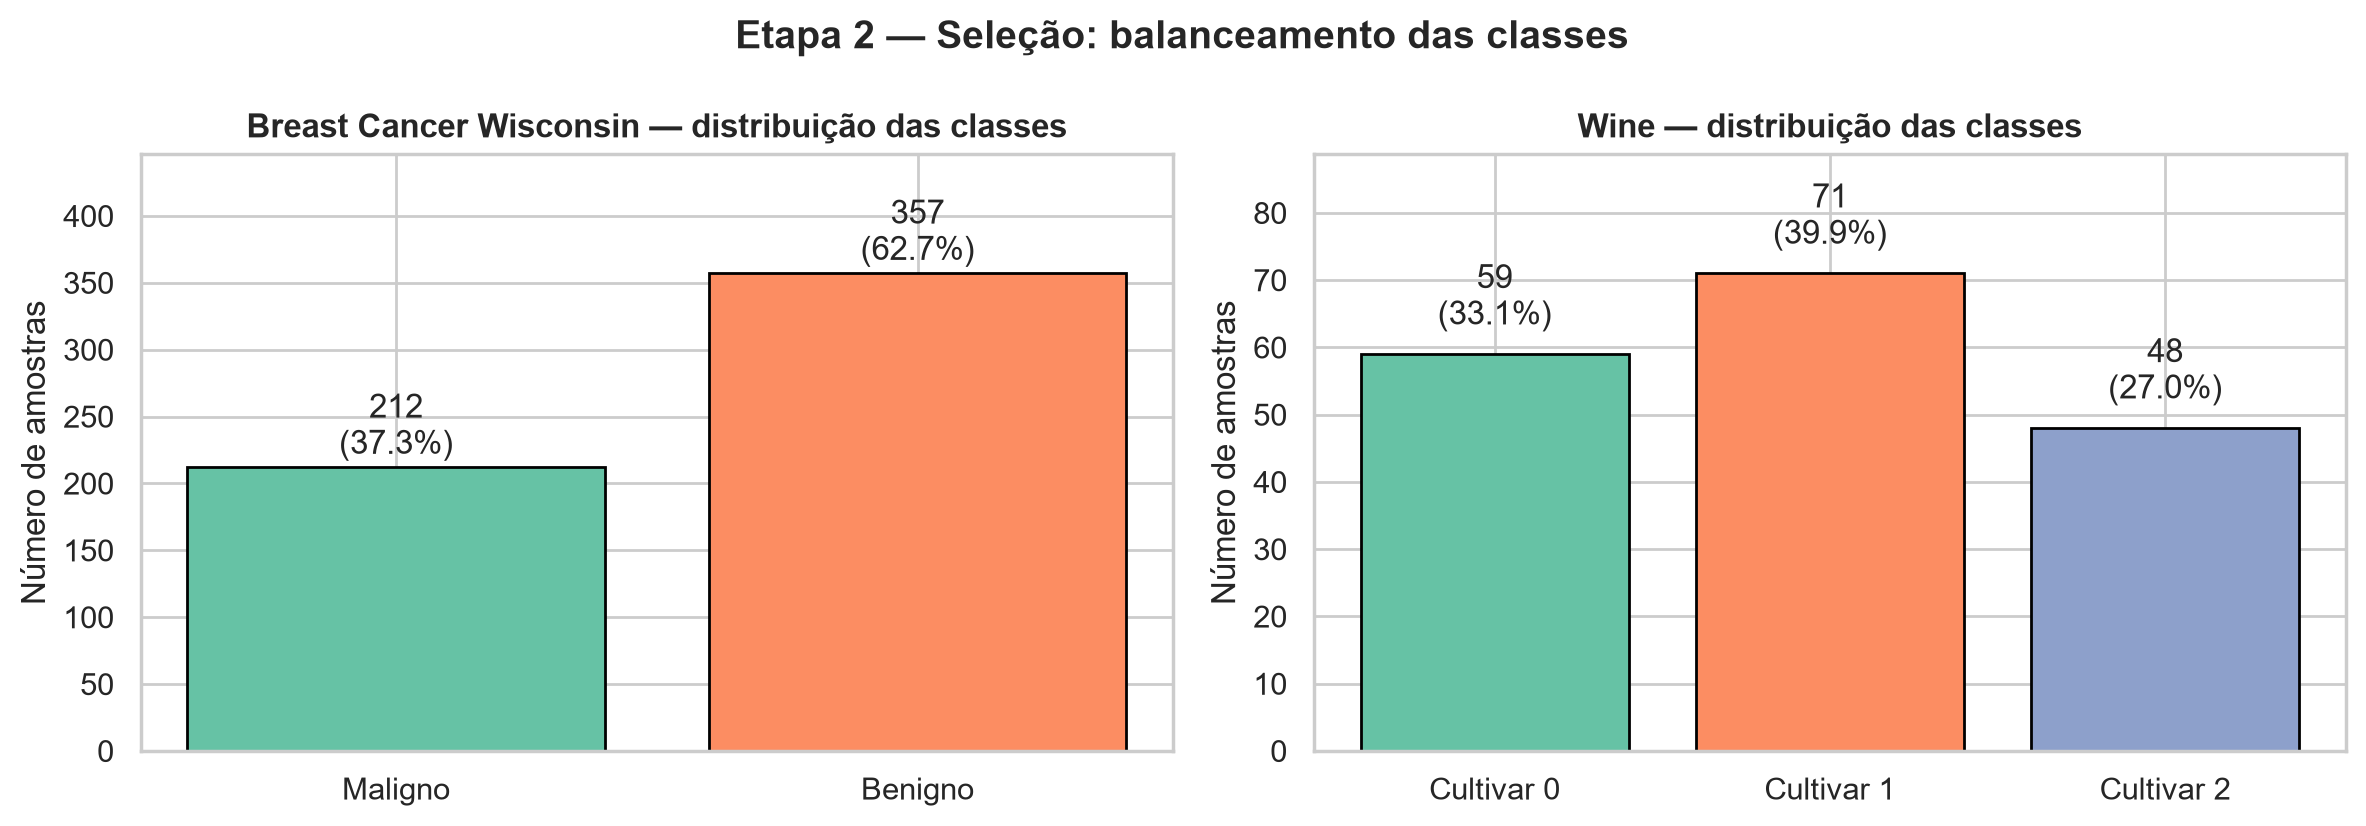
\includegraphics[width=\textwidth, keepaspectratio]{figuras/E2_distribuicao_classes.png}
    \caption{Distribuição das classes nos conjuntos Breast Cancer Wisconsin e Wine.}
    \label{fig:distribuicao_classes}
\end{figure}

\section{ETAPA 3: PRÉ-PROCESSAMENTO}

\subsection{QUALIDADE DOS DADOS}

Não foram encontrados valores ausentes, linhas duplicadas, atributos constantes nem valores negativos, portanto nenhuma limpeza de registros foi necessária. Por outro lado, a razão entre o maior e o menor desvio padrão dos atributos é de 215.170,7 no Breast Cancer (por exemplo, \texttt{area} contra \texttt{smoothness}) e de 2.530,3 no Wine (\texttt{proline} contra \texttt{hue}). Os atributos estão, portanto, em escalas muito diferentes, o que torna a padronização obrigatória para os métodos baseados em distância (KNN, grafos de vizinhança, K-Médias e DBSCAN).

\subsection{\textit{OUTLIERS}}

Pelo critério de Tukey (1,5 $\times$ IQR), 30,1\% das amostras do Breast Cancer possuem pelo menos um atributo \textit{outlier}, e elas se concentram fortemente na classe maligna (53,8\% dos malignos, contra 16,0\% dos benignos). Tumores malignos têm núcleos maiores e mais irregulares, de modo que valores extremos de área, raio e concavidade são \textbf{informação diagnóstica, e não ruído}. Removê-los apagaria justamente os casos mais típicos de malignidade. No Wine, apenas 9,6\% das amostras possuem algum \textit{outlier}. \textbf{Decisão: os \textit{outliers} foram mantidos} nos dois conjuntos.

\subsection{RELEVÂNCIA E SEPARABILIDADE DOS ATRIBUTOS}

A relevância de cada atributo foi medida pela estatística F da ANOVA e pela informação mútua com a classe. As duas medidas produzem rankings muito parecidos (correlação de Spearman de 0,957 no Breast Cancer e 0,951 no Wine). Os atributos mais relevantes são \texttt{worst concave points}, \texttt{worst perimeter} e \texttt{mean concave points} no Breast Cancer, e \texttt{flavanoids}, \texttt{proline} e \texttt{od280/od315} no Wine.

As Figuras \ref{fig:boxplots_bc} e \ref{fig:boxplots_wine} mostram a distribuição, por classe, de três atributos fortemente discriminativos de cada base, os mesmos usados na apresentação. No Breast Cancer, há um intervalo vazio entre o 3º quartil dos benignos e o 1º quartil dos malignos (``zona de segurança''): 13,4 a 15,1 para \texttt{mean radius}, 0,033 a 0,065 para \texttt{mean concave points} e 86 a 99 para \texttt{mean perimeter}. Quanto maior essa distância, maior a margem para o modelo acertar sem confundir os diagnósticos. Por outro lado, os bigodes das duas classes se cruzam, o que caracteriza casos ambíguos e o risco de falsos negativos quando se usa uma única variável. O uso conjunto dos 30 atributos atenua essa ambiguidade.

\begin{figure}[htbp]
    \centering
    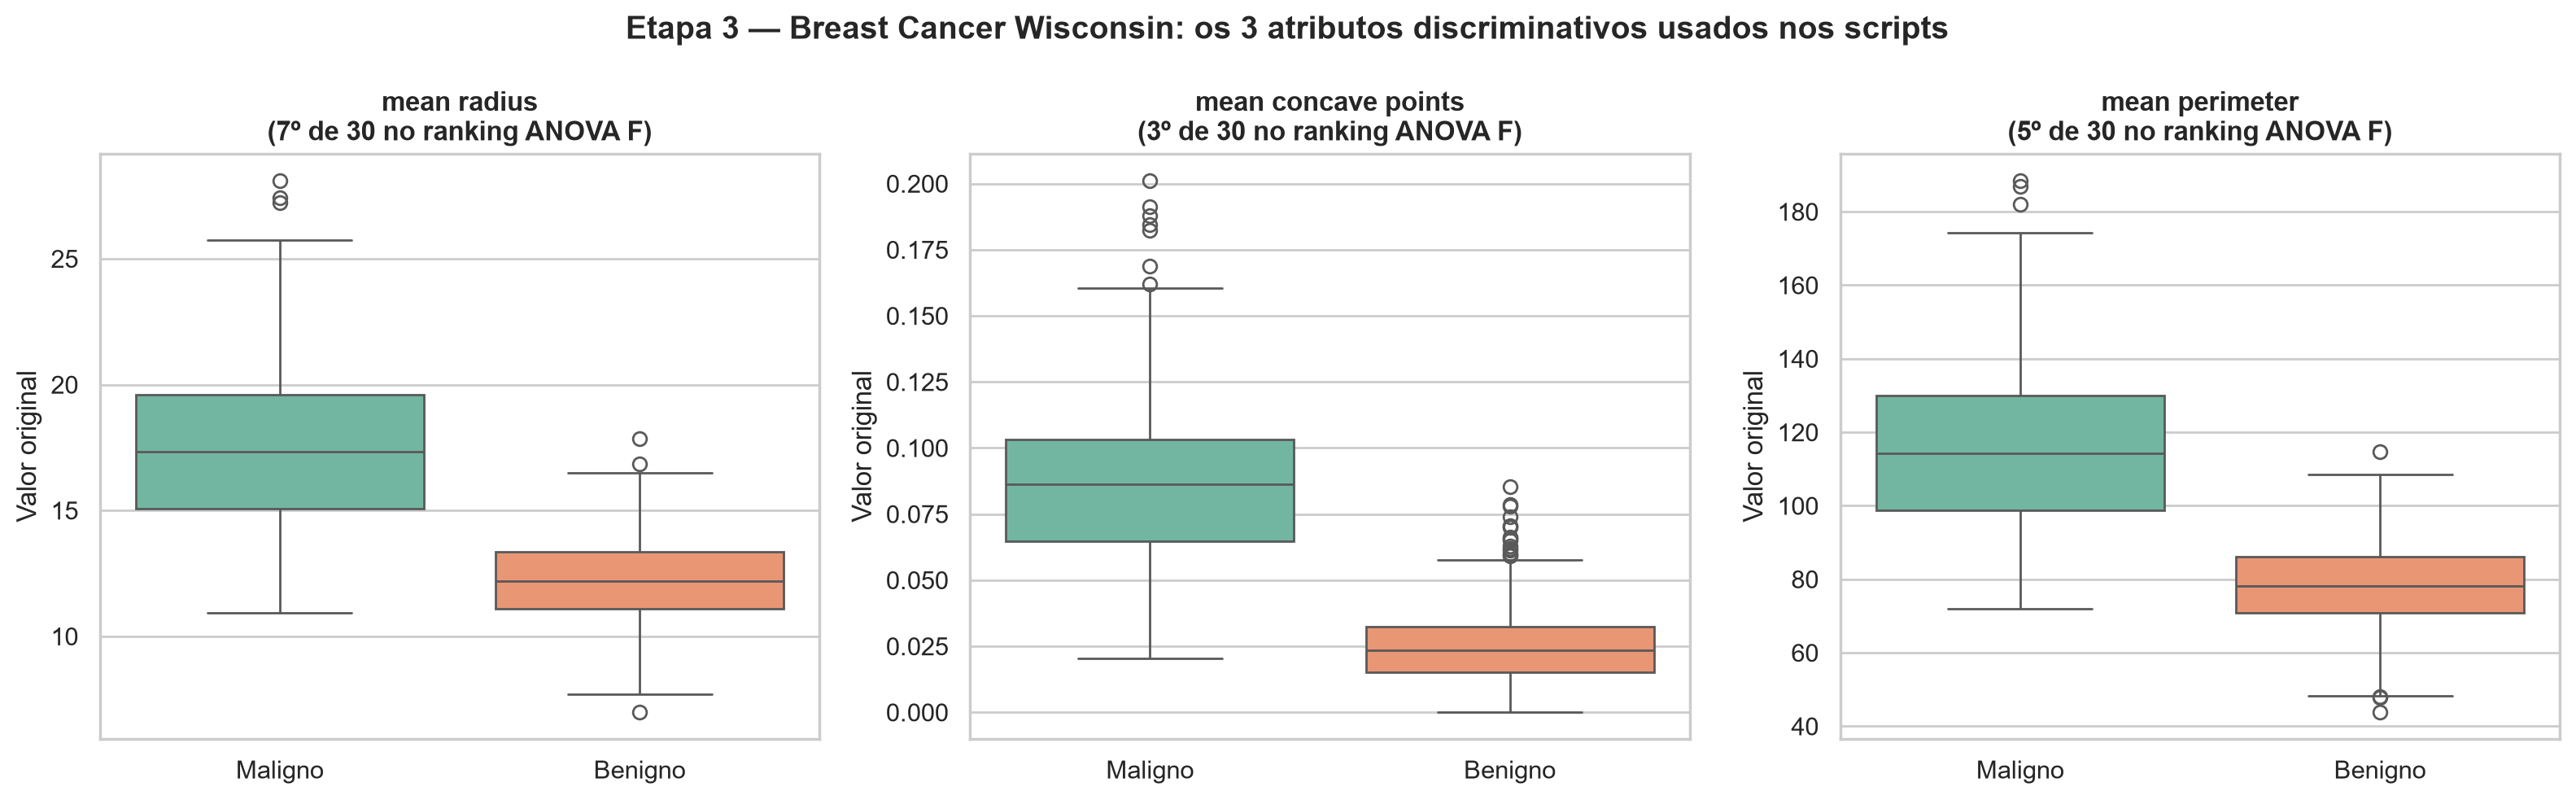
\includegraphics[width=\textwidth, keepaspectratio]{figuras/E3_breast_cancer_atributos_scripts.png}
    \caption{Breast Cancer Wisconsin: distribuição de \texttt{mean radius}, \texttt{mean concave points} e \texttt{mean perimeter} por classe. Os títulos indicam a posição de cada atributo no ranking da ANOVA.}
    \label{fig:boxplots_bc}
\end{figure}

No Wine, \texttt{flavanoids} separa bem as três cultivares, com intervalos vazios de 2,48 a 2,68 (entre as cultivares 1 e 0) e de 0,92 a 1,60 (entre as cultivares 2 e 1). Já \texttt{color\_intensity} e \texttt{alcohol} separam bem a cultivar 1 das demais (intervalos de 3,40 a 4,55 e de 12,52 a 12,80, respectivamente), mas apresentam sobreposição entre as cultivares 0 e 2. O problema multiclasse exige, portanto, a combinação dos atributos, com \texttt{flavanoids} atuando como critério de desempate.

\begin{figure}[htbp]
    \centering
    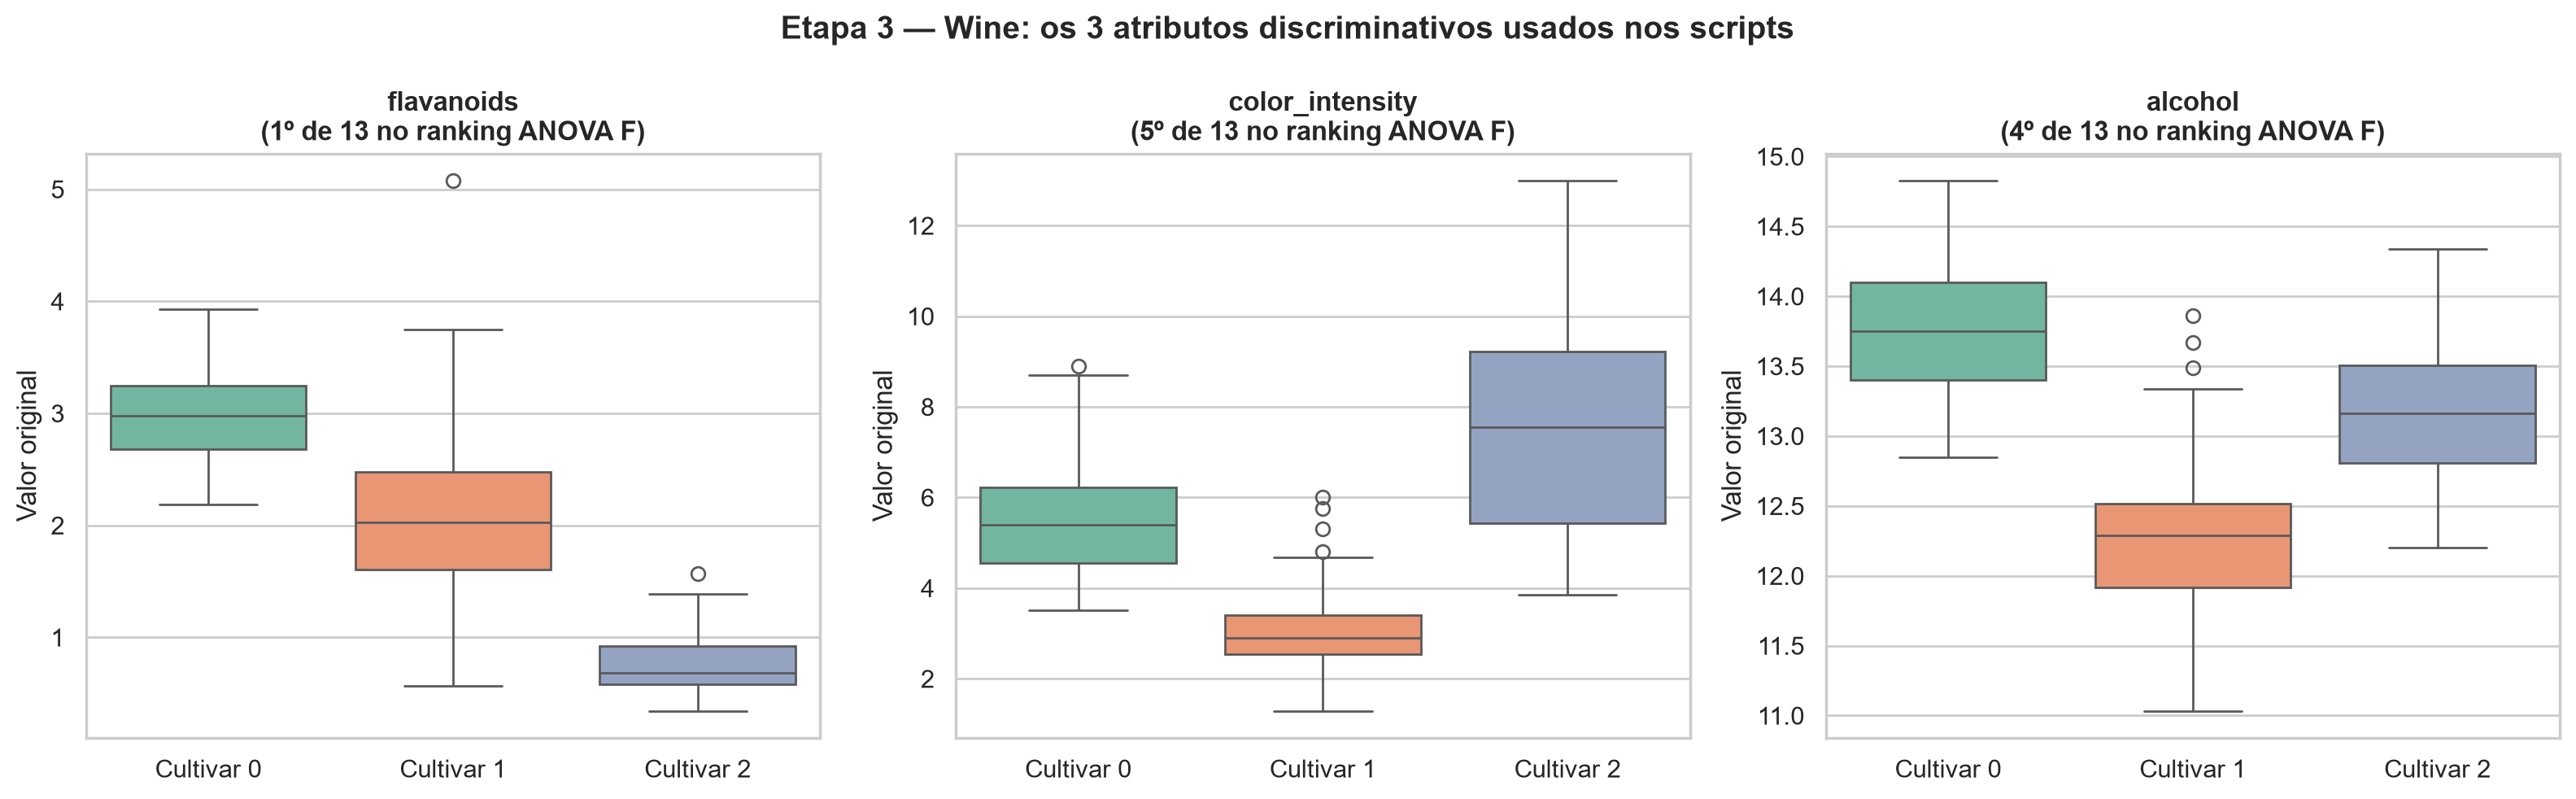
\includegraphics[width=\textwidth, keepaspectratio]{figuras/E3_wine_atributos_scripts.png}
    \caption{Wine: distribuição de \texttt{flavanoids}, \texttt{color\_intensity} e \texttt{alcohol} por cultivar.}
    \label{fig:boxplots_wine}
\end{figure}

\subsection{CORRELAÇÃO ENTRE ATRIBUTOS}

O Breast Cancer apresenta forte redundância: 21 pares de atributos têm correlação $|r| > 0{,}9$. Raio, perímetro e área carregam praticamente a mesma informação ($r \approx 0{,}99$). No Wine, nenhum par ultrapassa esse limite.

\subsection{PARTIÇÃO TREINO/TESTE E PADRONIZAÇÃO}

Antes de qualquer ajuste estatístico, 25\% de cada conjunto foram separados, de forma estratificada, para teste. O conjunto de teste ficou isolado e foi usado apenas para medir o desempenho final. Toda decisão que alimenta os modelos (padronização, PCA e hiperparâmetros) foi ajustada somente no treino.

Para escolher o escalonamento, foi comparado, por validação cruzada estratificada de 5 \textit{folds} no treino, o efeito de quatro opções no KNN ($k = 5$) e na Regressão Logística (Figura \ref{fig:padronizacao} e Tabela \ref{tab:padronizacao}). O escalonador foi ajustado dentro do \textit{pipeline} a cada \textit{fold}, sem vazamento de informação.

\begin{table}[htbp]
\centering
\caption{F1-macro médio (validação cruzada de 5 \textit{folds}) para diferentes escalonamentos.}
\label{tab:padronizacao}
\footnotesize
\begin{tabular}{llcccc}
\toprule
\textbf{Base} & \textbf{Modelo} & \textbf{Nenhum} & \textbf{Standard} & \textbf{MinMax} & \textbf{Robust} \\
\midrule
\multirow{2}{*}{Breast Cancer} & KNN ($k=5$) & 0,934 & 0,964 & 0,967 & 0,959 \\
 & Reg. Logística & 0,942 & 0,977 & 0,969 & 0,975 \\
\midrule
\multirow{2}{*}{Wine} & KNN ($k=5$) & 0,632 & 0,956 & 0,970 & 0,942 \\
 & Reg. Logística & 0,971 & 0,978 & 0,985 & 0,985 \\
\bottomrule
\end{tabular}
\end{table}

\begin{figure}[htbp]
    \centering
    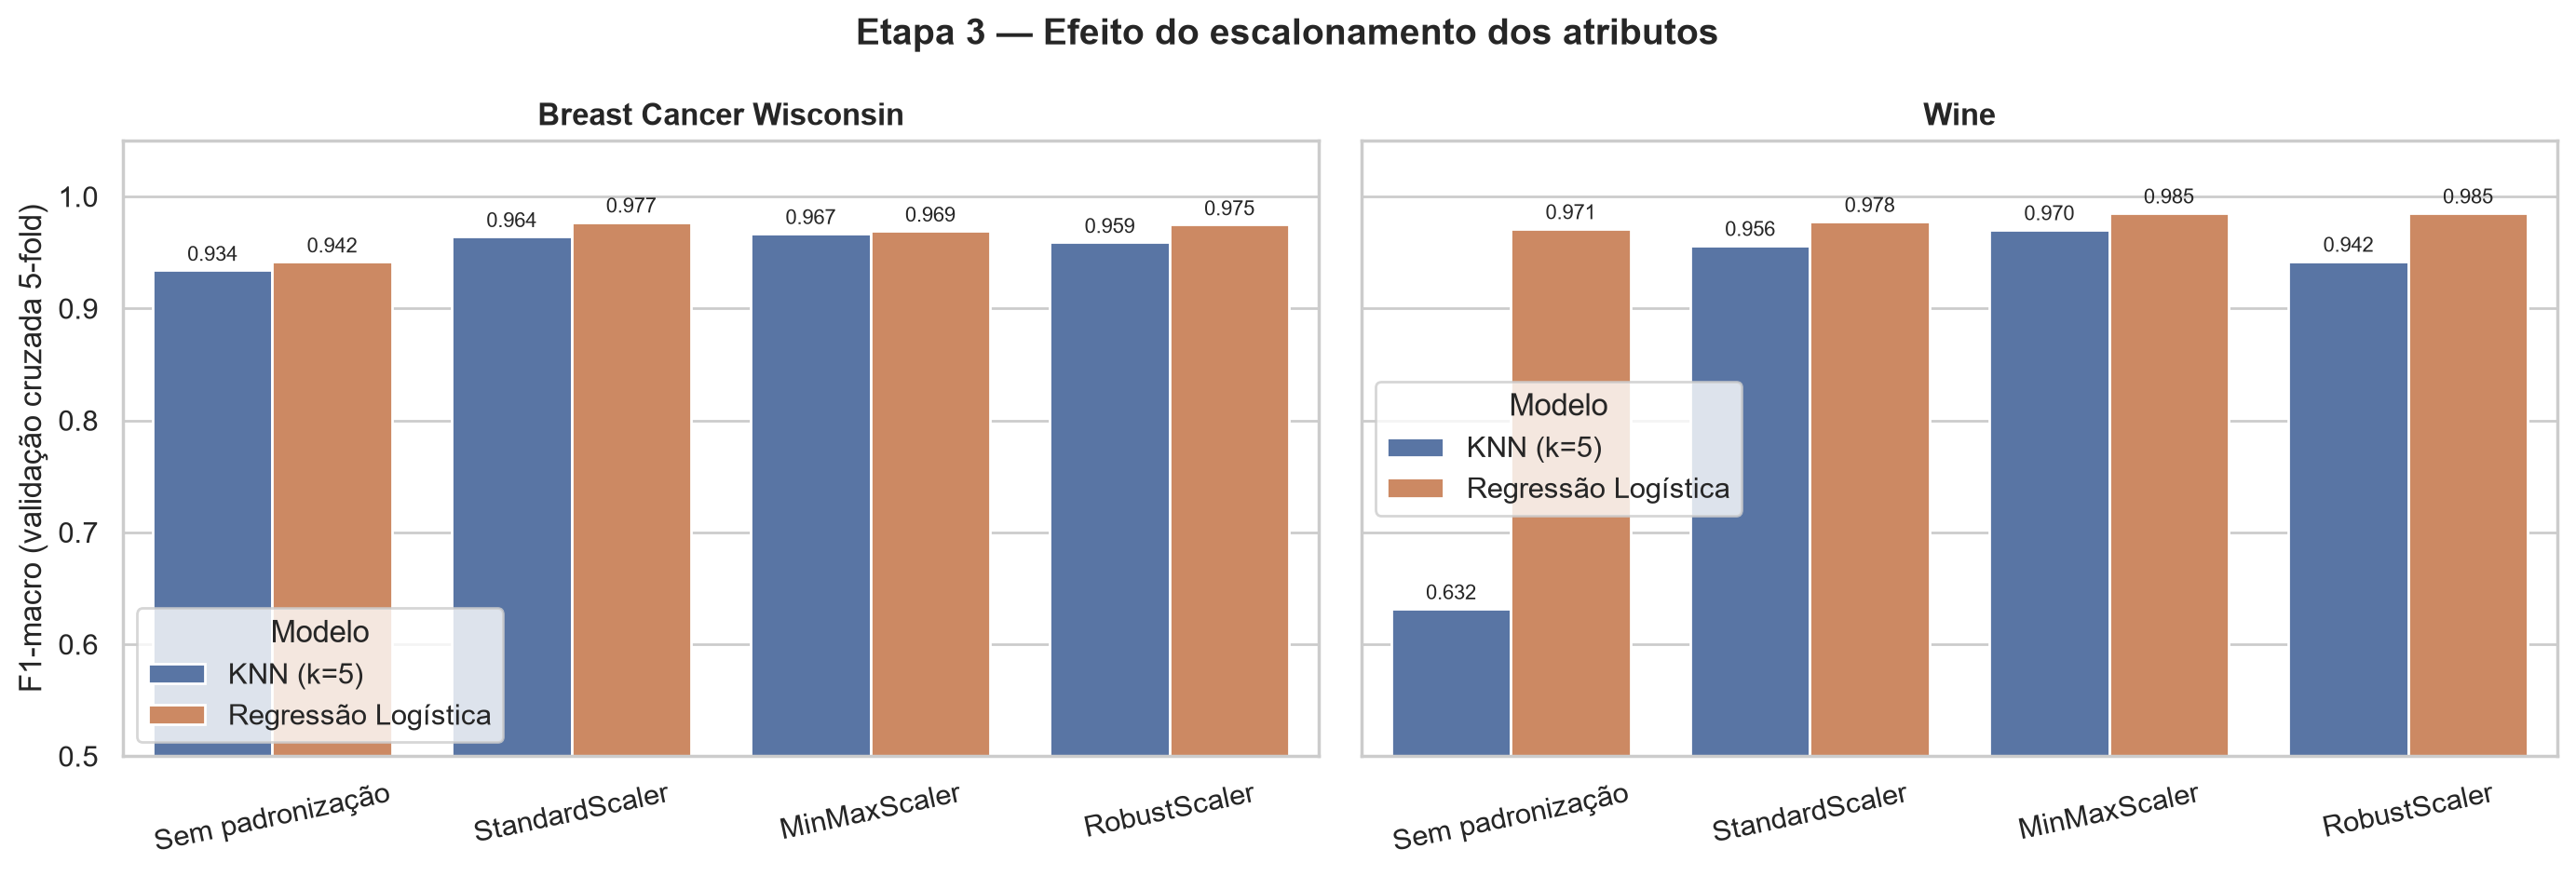
\includegraphics[width=\textwidth, keepaspectratio]{figuras/E3_efeito_padronizacao.png}
    \caption{Efeito do escalonamento no F1-macro do KNN e da Regressão Logística (validação cruzada no treino).}
    \label{fig:padronizacao}
\end{figure}

O escalonamento é decisivo para o KNN no Wine: o F1 sobe de 0,632, sem padronização, para 0,956 com o \texttt{StandardScaler}. Sem escalonamento, a distância euclidiana é dominada por \texttt{proline} (desvio padrão $\approx$ 315) e \texttt{magnesium} ($\approx$ 14). Entre os escalonadores, as diferenças ficam dentro de um desvio padrão da validação cruzada. \textbf{Decisão: \texttt{StandardScaler}}, pois não perde de forma consistente para os demais e deixa todos os atributos com média zero e variância unitária. Com isso, o PCA da Etapa 4 equivale ao PCA da matriz de correlação, e nenhuma unidade de medida domina as componentes.

\section{ETAPA 4: TRANSFORMAÇÃO}

Foram investigadas duas representações de baixa dimensão, ambas não supervisionadas e ajustadas apenas no treino padronizado: o PCA, linear, e os \textit{Laplacian Eigenmaps}, não lineares e baseados em grafo de vizinhança. A Tabela \ref{tab:pca} resume a variância explicada pelo PCA.

\begin{table}[htbp]
\centering
\caption{Variância explicada pelo PCA no treino padronizado.}
\label{tab:pca}
\footnotesize
\begin{tabular}{lcccccc}
\toprule
\textbf{Base} & \textbf{PC1} & \textbf{PC2} & \textbf{PC1+PC2} & \textbf{CPs p/ 90\%} & \textbf{CPs p/ 95\%} & \textbf{Dim. original} \\
\midrule
Breast Cancer & 43,9\% & 19,5\% & 63,4\% & 7 & 10 & 30 \\
Wine & 35,7\% & 19,2\% & 55,0\% & 8 & 10 & 13 \\
\bottomrule
\end{tabular}
\end{table}

A redundância observada no Breast Cancer faz com que a PC1 sozinha concentre 43,9\% da variância. No biplot da Figura \ref{fig:biplot_bc}, a PC1 aponta na direção dos atributos de \textbf{tamanho} (raio, perímetro e área), e os tumores malignos ocupam a região de PC1 alto. A PC2 é dominada pela dimensão fractal, quase ortogonal ao diagnóstico. No Wine, a variância é mais distribuída entre as componentes.

\begin{figure}[htbp]
    \centering
    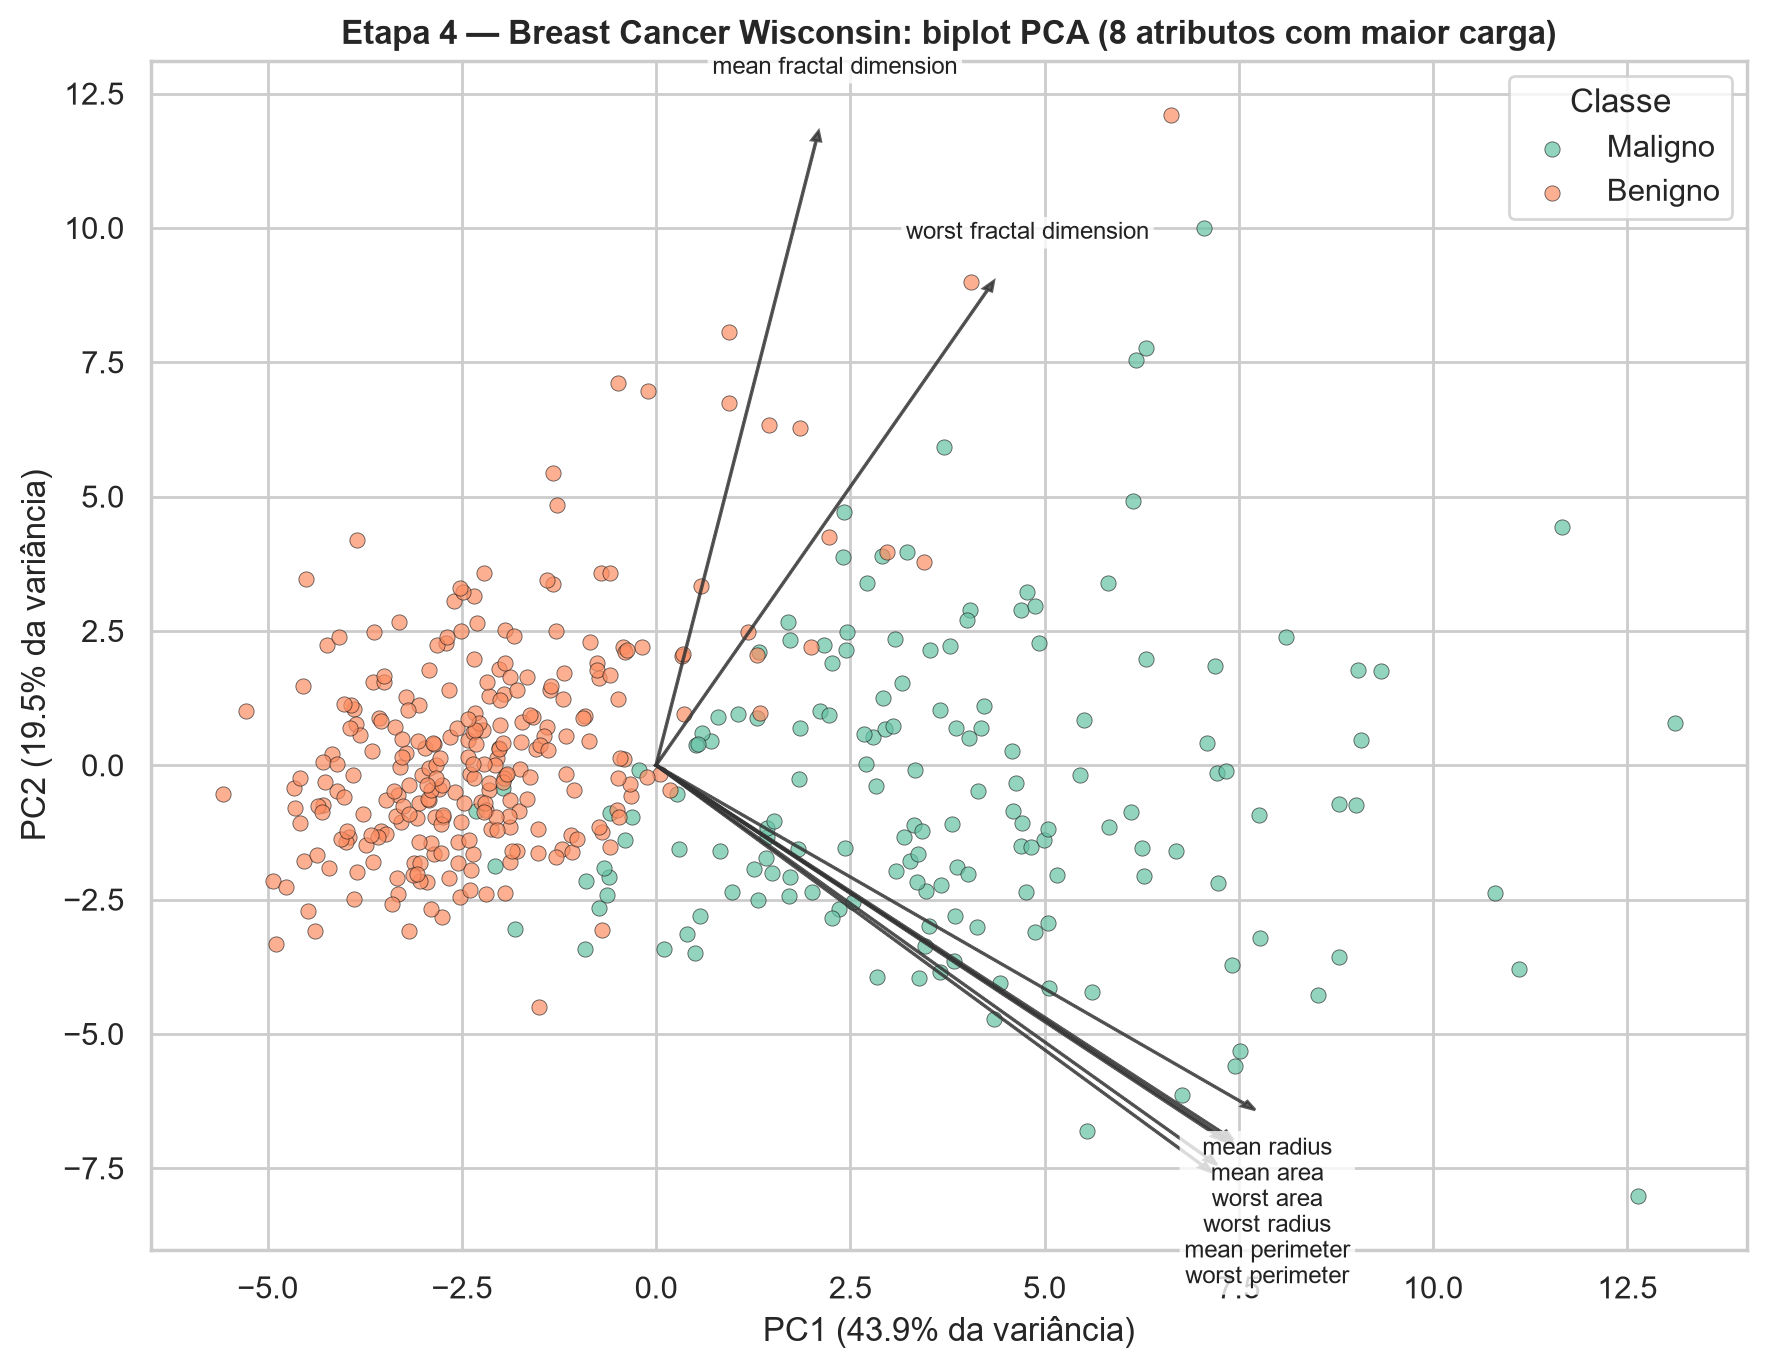
\includegraphics[width=0.85\textwidth, keepaspectratio]{figuras/E4_breast_cancer_pca_biplot.png}
    \caption{Breast Cancer Wisconsin: projeção PCA 2D do treino e cargas (\textit{loadings}) dos atributos mais relevantes.}
    \label{fig:biplot_bc}
\end{figure}

Para medir quanto da separabilidade das classes cada representação preserva, foram calculadas a silhueta das classes reais e o F1-macro de um KNN ($k = 5$) em validação cruzada (Figura \ref{fig:separabilidade}). No Wine, o KNN no PCA 2D (F1 = 0,978) chega a superar o espaço completo (0,963), pois as dimensões descartadas carregam mais ruído do que sinal. No Breast Cancer, a perda é pequena (de 0,962 para 0,932). A silhueta das classes reais aumenta nas projeções 2D (no Wine, de 0,281 para 0,542 no PCA e 0,767 nos \textit{Laplacian Eigenmaps}). Isso indica que, no espaço completo, as distâncias são ``diluídas'' por atributos pouco discriminativos, efeito que prejudica os métodos baseados em densidade. Os grupos muito compactos obtidos pelos \textit{Laplacian Eigenmaps} no Wine indicam que a hipótese de \textit{cluster} vale bem nessa base.

\begin{figure}[htbp]
    \centering
    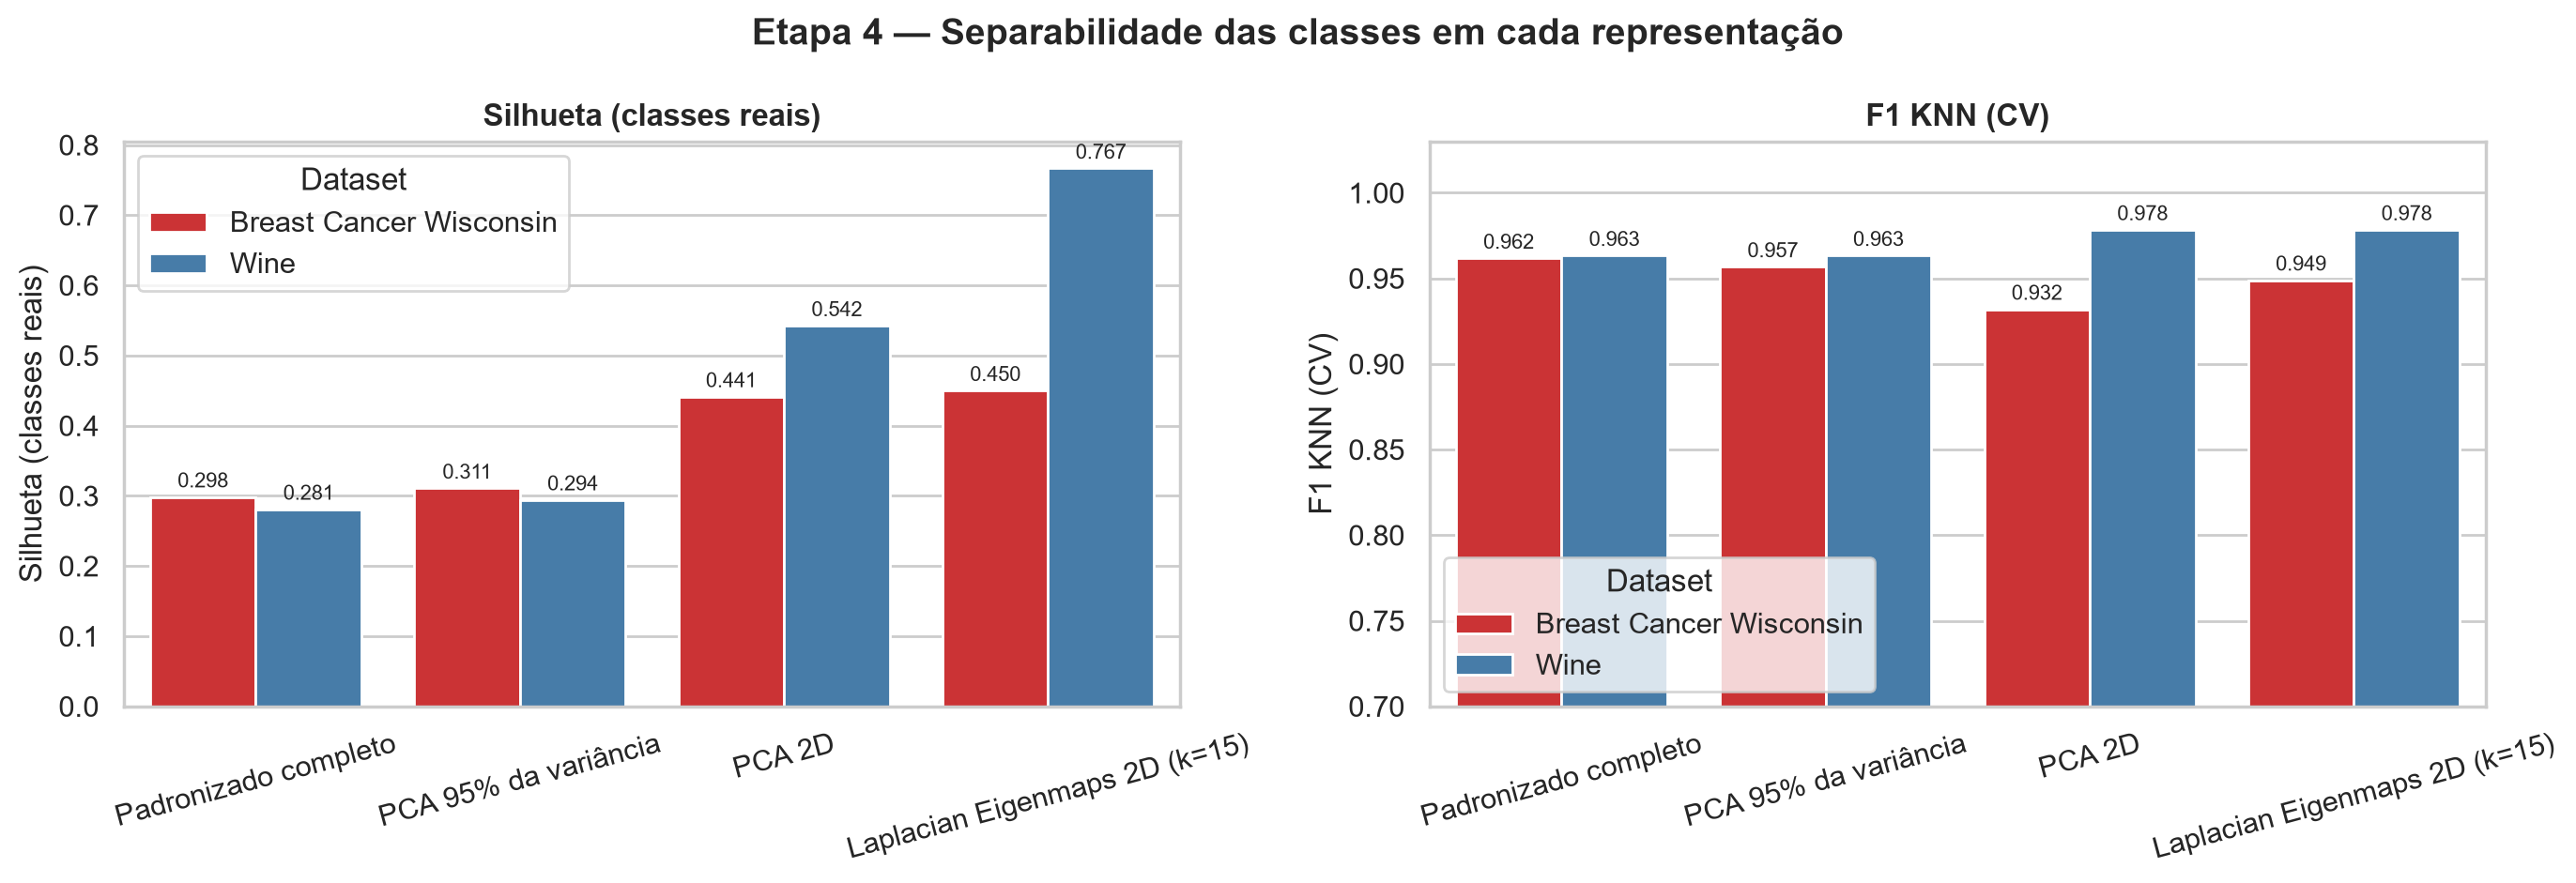
\includegraphics[width=\textwidth, keepaspectratio]{figuras/E4_separabilidade_representacoes.png}
    \caption{Separabilidade das classes em cada representação: silhueta das classes reais e F1-macro do KNN em validação cruzada.}
    \label{fig:separabilidade}
\end{figure}

\textbf{Decisão:} os classificadores e os agrupamentos trabalham no \textbf{espaço padronizado completo}, sem perda de informação. As projeções 2D são usadas apenas para visualização.

\section{PROTOCOLO EXPERIMENTAL DA ETAPA 5}

O agrupamento foi aplicado ao treino padronizado \textbf{sem nenhum rótulo}. Os rótulos verdadeiros foram usados somente para avaliar os agrupamentos.

Na classificação semi-supervisionada, para cada taxa e repetição, uma fração estratificada dos pontos de treino manteve o rótulo e os demais foram marcados como não rotulados. Em cada repetição, todos os modelos receberam \textbf{o mesmo} subconjunto rotulado, o que permite comparações pareadas. Os \textit{baselines} foram treinados apenas com os pontos rotulados, enquanto os semi-supervisionados usaram também os não rotulados. A avaliação principal foi feita no conjunto de teste isolado. O sorteio estratificado evita que uma classe inteira fique sem nenhum ponto rotulado; no Wine, em que 5\% do treino correspondem a apenas 7 amostras, foi imposto ainda um mínimo de dois pontos rotulados por cultivar. Os dois \textit{scripts} adotaram protocolos ligeiramente diferentes, resumidos na Tabela \ref{tab:protocolo}.

\begin{table}[htbp]
\centering
\caption{Protocolo experimental de cada conjunto de dados.}
\label{tab:protocolo}
\footnotesize
\begin{tabular}{p{3.0cm} p{5.6cm} p{5.6cm}}
\toprule
\textbf{Item} & \textbf{Breast Cancer Wisconsin} & \textbf{Wine} \\
\midrule
Taxas de rótulos & 0,05; 0,10; 0,20; 0,30; 0,40; 0,50; 0,60; 0,70 & 0,05; 0,10; 0,20; 0,30; 0,50; 0,70 \\
\addlinespace
Repetições & 5 (sementes 10, 20, 30, 40 e 50) & 10 (sementes 100 a 109) \\
\addlinespace
Sorteio dos rotulados & Estratificado & Estratificado, com no mínimo 2 por classe \\
\addlinespace
\textit{Baselines} & KNN ($k = 5$); Regressão Logística & KNN ($k = \min(5, n_{\text{rot}}/2)$); Regressão Logística \\
\addlinespace
Semi-supervisionados & \textit{Label Spreading} (grafo kNN, $k = 7$); \textit{Self-Training} com RL (limiar 0,75) & \textit{Label Spreading} e \textit{Label Propagation} (RBF, $\gamma = 1/13$); \textit{Self-Training} com RL (limiar 0,80) \\
\addlinespace
K-Médias & $k = 2$, \texttt{n\_init} = 10 & $k = 3$, \texttt{n\_init} = 20 \\
\addlinespace
DBSCAN & \texttt{eps} = 4,5; \texttt{min\_samples} = 5 & \texttt{eps} = 2,3; \texttt{min\_samples} = 4 \\
\bottomrule
\end{tabular}
\end{table}
